\documentclass[10pt,letterpaper]{article}

\usepackage[margin=0.78in]{geometry}
\usepackage[hidelinks]{hyperref}
\usepackage{booktabs}
\usepackage{tabularx}
\usepackage{enumitem}
\usepackage{xcolor}
\usepackage{titlesec}
\usepackage{tikz}
\usetikzlibrary{arrows.meta,positioning,fit,calc}
\newcolumntype{Y}{>{\centering\arraybackslash}X}

\definecolor{ink}{HTML}{111827}
\definecolor{muted}{HTML}{4B5563}
\definecolor{blue}{HTML}{2563EB}
\definecolor{green}{HTML}{059669}
\definecolor{orange}{HTML}{EA580C}
\definecolor{purple}{HTML}{7C3AED}
\definecolor{panel}{HTML}{F8FAFC}

\setlength{\parindent}{0pt}
\setlength{\parskip}{4pt}
\titleformat{\section}{\large\bfseries\color{ink}}{\thesection}{0.6em}{}
\titleformat{\subsection}{\normalsize\bfseries\color{ink}}{\thesubsection}{0.6em}{}
\setlist[itemize]{leftmargin=1.25em,itemsep=2pt,topsep=2pt}

\newcommand{\metric}[3]{
  \begin{minipage}[t]{0.22\linewidth}
  \centering
  {\Large \textbf{\color{blue}#1}}\\
  {\small \textbf{#2}}\\
  {\scriptsize \color{muted}#3}
  \end{minipage}
}

\begin{document}

\begin{center}
{\LARGE \textbf{Algorithmic Supervision of High-Frequency Financial Flows}}\\
\vspace{2pt}
{\large A Permissioned Blockchain and Agent-Based Simulation for AML Compliance in Nepal}\\
\vspace{4pt}
\textbf{Dikshant Pandey}\\
Kathmandu, Nepal\\
January 30, 2026\\
\vspace{3pt}
Version 2.0: 100k transaction reproducible simulation
\end{center}

\begin{abstract}
\noindent This research presents the Nepal Compliance Ledger (NCL), a regulatory technology prototype for supervising high-frequency financial flows before settlement. The updated implementation combines an agent-based transaction market, sliding-window velocity checks, bounded graph-cycle detection, and a permissioned blockchain audit layer with Merkle roots, hash-linked blocks, policy-version binding, and validator quorum signatures. A deterministic simulation with 10,000 agents and 100,000 transactions produced 38,566 true positives, 39 false positives, 6,601 false negatives, and 54,794 true negatives. The system achieved 99.90\% precision, 85.39\% recall, and an F1 score of 0.9207 while sealing 196 auditable blocks with intact chain verification. These results suggest that a hub-and-spoke compliance ledger can reduce AML latency while preserving a tamper-evident regulatory audit trail.
\end{abstract}

\section{Introduction}

Anti-money laundering (AML) enforcement in developing financial systems faces a timing problem. Suspicious flows are often detected after settlement, after funds have already moved across institutions or been fragmented into low-value transfers. Structuring, also known as smurfing, exploits this weakness by splitting a larger illicit amount into many smaller transactions that sit below scalar reporting thresholds.

NCL reframes the problem as one of transaction velocity and graph topology. Instead of asking only whether a single payment exceeds a threshold, the system evaluates whether a sender is moving too frequently inside a rolling time window and whether a new edge closes a short circular path. The updated implementation also records every compliance decision into a permissioned blockchain-style ledger so that banks and regulators can audit a shared, tamper-evident history.

\section{Methodology}

\subsection{Hub-and-Spoke Architecture}

The project preserves the original hub-and-spoke design: commercial nodes submit transaction requests, a regulatory compliance brain evaluates them, clean transactions proceed to participating banks, and every decision is written into an immutable audit ledger with a regulator dashboard feed.

\begin{center}
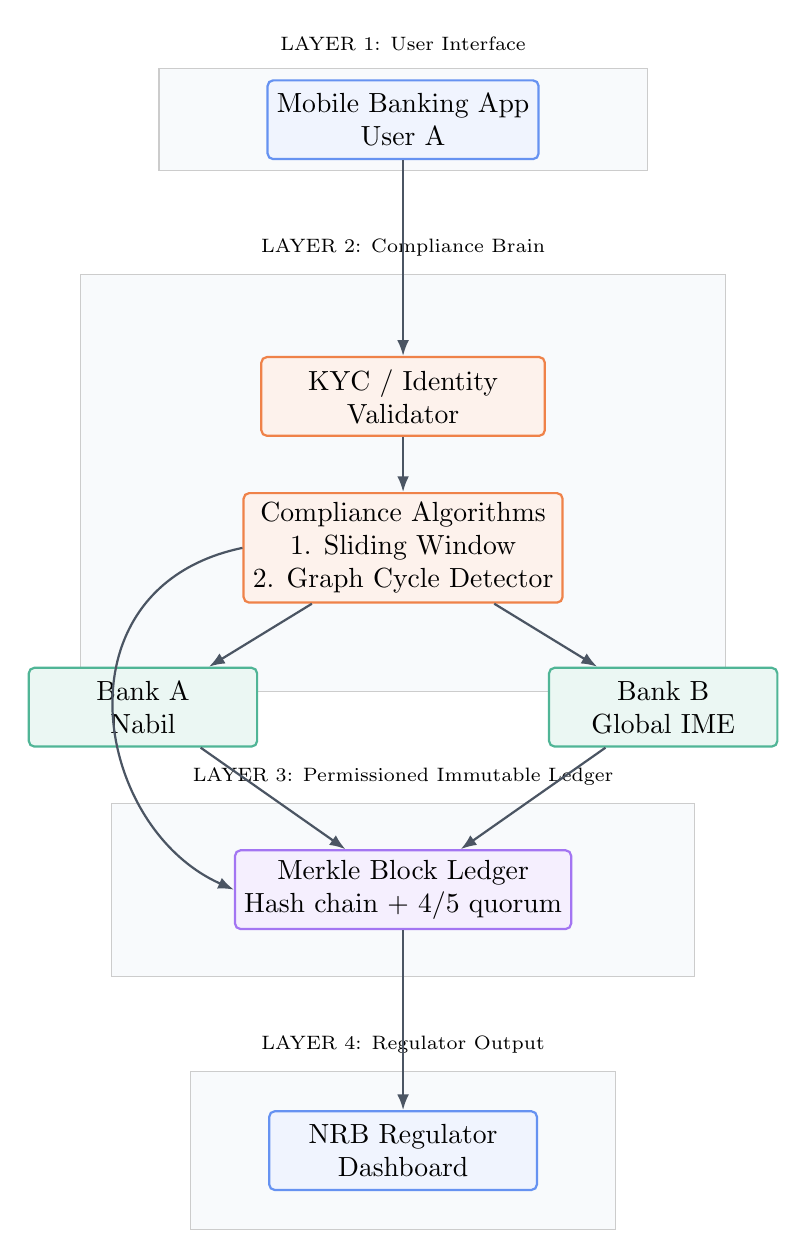
\begin{tikzpicture}[
  node distance=7mm,
  layer/.style={rectangle, draw=black!20, fill=panel, minimum width=62mm, minimum height=13mm, align=center},
  boxblue/.style={rectangle, rounded corners=2pt, draw=blue!70, fill=blue!7, thick, minimum width=34mm, minimum height=10mm, align=center},
  boxorange/.style={rectangle, rounded corners=2pt, draw=orange!75, fill=orange!8, thick, minimum width=36mm, minimum height=10mm, align=center},
  boxgreen/.style={rectangle, rounded corners=2pt, draw=green!70, fill=green!8, thick, minimum width=29mm, minimum height=10mm, align=center},
  boxpurple/.style={rectangle, rounded corners=2pt, draw=purple!70, fill=purple!8, thick, minimum width=40mm, minimum height=10mm, align=center},
  arrow/.style={-{Latex[length=2mm]}, thick, draw=muted}
]
\node[layer] (uiLayer) {};
\node[boxblue] (ui) at (uiLayer.center) {Mobile Banking App\\User A};
\node[above=1mm of uiLayer] {\scriptsize LAYER 1: User Interface};

\node[layer, below=13mm of uiLayer, minimum height=53mm, minimum width=82mm] (brainLayer) {};
\node[above=1mm of brainLayer] {\scriptsize LAYER 2: Compliance Brain};
\node[boxorange] (kyc) at ($(brainLayer.center)+(0,11mm)$) {KYC / Identity\\Validator};
\node[boxorange, below=7mm of kyc] (engine) {Compliance Algorithms\\1. Sliding Window\\2. Graph Cycle Detector};
\node[boxgreen, below left=8mm and -2mm of engine] (bankA) {Bank A\\Nabil};
\node[boxgreen, below right=8mm and -2mm of engine] (bankB) {Bank B\\Global IME};

\node[layer, below=14mm of brainLayer, minimum height=22mm, minimum width=74mm] (ledgerLayer) {};
\node[above=1mm of ledgerLayer] {\scriptsize LAYER 3: Permissioned Immutable Ledger};
\node[boxpurple] (ledger) at (ledgerLayer.center) {Merkle Block Ledger\\Hash chain + 4/5 quorum};

\node[layer, below=12mm of ledgerLayer, minimum height=20mm, minimum width=54mm] (auditLayer) {};
\node[above=1mm of auditLayer] {\scriptsize LAYER 4: Regulator Output};
\node[boxblue] (dash) at (auditLayer.center) {NRB Regulator\\Dashboard};

\draw[arrow] (ui) -- (kyc);
\draw[arrow] (kyc) -- (engine);
\draw[arrow] (engine) -- (bankA);
\draw[arrow] (engine) -- (bankB);
\draw[arrow] (engine.west) .. controls +(-24mm,-5mm) and +(-18mm,8mm) .. (ledger.west);
\draw[arrow] (bankA) -- (ledger);
\draw[arrow] (bankB) -- (ledger);
\draw[arrow] (ledger) -- (dash);
\end{tikzpicture}

Figure 1: NCL hub-and-spoke architecture, preserving the original system design while replacing the append-only log with a permissioned block ledger.
\end{center}

\subsection{Sliding-Window Velocity Protocol}

For each sender $a$, the engine stores a rolling log of recent transaction times. A transaction at time $T$ is blocked when the number of transactions in the last $W$ seconds exceeds a policy threshold $\tau$:

\[
\mathrm{VelocityCount}(a,T)=\sum_i \mathbf{1}(T-t_i < W)
\]

In the implementation, $W=300$ seconds and $\tau=5$. A deque-backed log is used so outdated timestamps are pruned in amortized constant time.

\subsection{Graph Cycle Detection}

Layering is modeled as a short cycle in the directed transaction graph. For a proposed edge $(u,v)$, NCL checks whether a path already exists from $v$ back to $u$ with depth at most $k$:

\[
v \rightarrow \cdots \rightarrow u,\quad |P| \leq k
\]

The implementation uses bounded DFS with $k=3$ and a 900-second graph memory window. This keeps the detector focused on recent circular flows rather than every historical transfer.

\subsection{Permissioned Blockchain Audit Layer}

The advanced implementation upgrades the earlier append-only ledger into a permissioned block ledger. Each transaction decision is converted into a canonical audit record and batched into blocks of 512 records. A block header contains:

\begin{itemize}
  \item previous block hash,
  \item Merkle root over transaction decision records,
  \item policy-version hash,
  \item proposer node,
  \item simulated validator signatures from a 4-of-5 quorum.
\end{itemize}

The chain verifier recomputes every Merkle root, block hash, previous-hash link, and quorum signature. A run is accepted only when the complete audit chain verifies as intact.

\section{Experimental Setup}

\begin{tabularx}{\linewidth}{@{}l X@{}}
\toprule
\textbf{Parameter} & \textbf{Value}\\
\midrule
Agents & 10,000 autonomous actors\\
Malicious population & 5\% of agents\\
Transaction volume & 100,000 transactions\\
Transaction mix & 55\% honest, 30\% structuring, 15\% ring-layering attempts\\
Sliding window & 300 seconds\\
Velocity threshold & 5 sender transactions per window\\
Cycle detector & Depth-3 DFS with 900-second graph memory\\
Ledger & 512-record blocks, SHA-256 hash chain, Merkle roots, 4-of-5 validator quorum\\
\bottomrule
\end{tabularx}

\section{Results}

\begin{center}
\fcolorbox{blue!20}{panel}{
\begin{minipage}{0.96\linewidth}
\metric{100,000}{Transactions}{deterministic ABM run}\hfill
\metric{99.90\%}{Precision}{39 false positives}\hfill
\metric{85.39\%}{Recall}{6,601 false negatives}\hfill
\metric{0.9207}{F1 Score}{balanced detection metric}
\end{minipage}}
\end{center}

\begin{tabularx}{\linewidth}{@{}l r@{\hspace{16mm}}l r@{}}
\toprule
\textbf{Confusion Matrix} & \textbf{Count} & \textbf{Ledger / Runtime} & \textbf{Value}\\
\midrule
True positives & 38,566 & Sealed blocks & 196\\
False positives & 39 & Block size & 512\\
False negatives & 6,601 & Validator quorum & 4/5\\
True negatives & 54,794 & Processing throughput & 102,948 tx/s\\
\bottomrule
\end{tabularx}

\vspace{4pt}
\begin{tabularx}{\linewidth}{@{}l r@{}}
\toprule
\textbf{Detection Breakdown} & \textbf{Count}\\
\midrule
Velocity flags & 38,271\\
Cycle flags & 334\\
Approved transactions & 61,395\\
Ledger chain integrity & Intact\\
\bottomrule
\end{tabularx}

\section{Discussion}

The upgraded simulation shows that most malicious activity is captured by velocity detection, while graph-cycle detection adds coverage for circular layering behavior. Precision remains high because honest users rarely exceed the rolling velocity threshold, and the bounded graph memory reduces accidental long-horizon cycle matches.

The ledger layer is not included for speed alone. Its purpose is institutional accountability. A centralized database can store the same rows, but a permissioned ledger creates a shared audit object: each block binds transaction decisions to a policy hash, previous block hash, Merkle root, and validator quorum. This makes later alteration detectable without requiring every participant to trust a single administrator.

\section{Limitations and Future Work}

\begin{itemize}
  \item The validator signatures are deterministic simulation signatures, not production cryptographic keys managed by real bank HSMs.
  \item The ABM uses synthetic behavior distributions; deployment would require calibration against legally shareable banking telemetry.
  \item The current graph detector uses bounded DFS; larger deployments should evaluate streaming graph anomaly methods.
  \item The policy engine is rules-first; a future version can add supervised risk scoring while keeping rule decisions explainable.
\end{itemize}

\section{Conclusion}

NCL demonstrates how real-time AML supervision can be represented as a pre-settlement compliance problem. The advanced implementation scales the simulation to 100,000 transactions and adds a permissioned blockchain audit layer with Merkle verification and validator quorum. The result is a research prototype that connects transaction monitoring, graph-based detection, and tamper-evident regulatory auditability in a single reproducible system.

\section*{References}
{\small
\begin{enumerate}[leftmargin=1.4em,itemsep=1pt]
  \item Financial Action Task Force. International Standards on Combating Money Laundering and the Financing of Terrorism and Proliferation.
  \item Nepal Rastra Bank. Unified Directives and AML/CFT supervisory guidance.
  \item Androulaki, E. et al. ``Hyperledger Fabric: A Distributed Operating System for Permissioned Blockchains.'' EuroSys, 2018.
  \item Nakamoto, S. ``Bitcoin: A Peer-to-Peer Electronic Cash System,'' 2008.
  \item Savage, D. et al. ``Detection of Money Laundering Groups Using Supervised Learning in Networks.'' arXiv:1608.00708, 2016.
\end{enumerate}
}

\end{document}
